\documentclass[tikz,border=12pt]{standalone}
% Shared visual language for standalone EMT block diagrams.
\usepackage{amsmath}
\usetikzlibrary{arrows.meta,backgrounds,calc,fit,positioning}

\tikzset{
    emt diagram/.style = {>={Stealth[length=2.4mm]}},
    line/.style        = {semithick, rounded corners=6pt},
    block/.style       = {draw, semithick, fill=white,
                          minimum height=1cm, minimum width=2.3cm},
    hblock/.style      = {block, minimum width=2.24cm, minimum height=1.3cm},
    vblock/.style      = {block, minimum width=1.3cm, minimum height=2.24cm},
    sum/.style         = {draw, semithick, fill=white, circle,
                          inner sep=2.6pt},
    signal/.style      = {circle, fill, inner sep=1.4pt,
                          label distance=3pt},
    sig/.style         = {font=\small},
    pm/.style          = {font=\scriptsize},
    wire jump/.style   = {line,
                          preaction={draw=white, line width=3pt,
                                     line cap=round}},
    enclosure/.style   = {draw, dashed, semithick, rounded corners=4pt},
    operator enclosure/.style = {enclosure, inner xsep=7mm, inner ysep=6mm}
}


\begin{document}
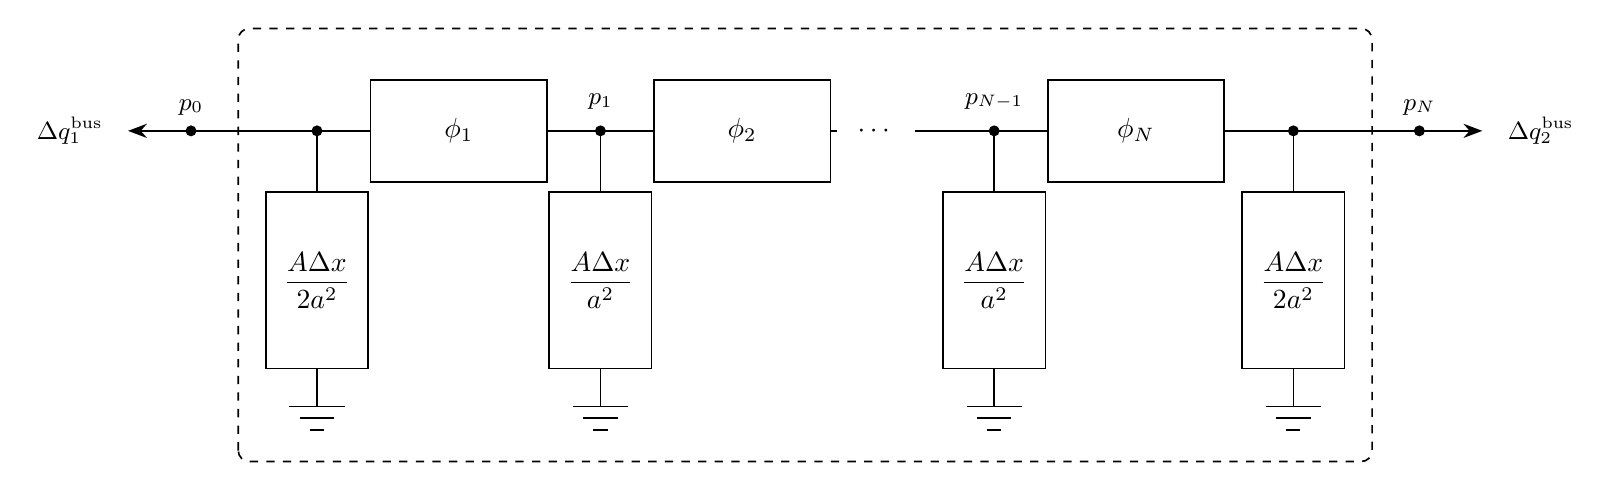
\begin{tikzpicture}[emt diagram]

% Segment blocks hold the mass fluxes; storage blocks sit at the nodes.
\node[hblock] (seg1) at (-4.4, 0) {$\phi_1$};
\node[hblock] (seg2) at (-0.8, 0) {$\phi_2$};
\node[hblock] (segN) at (4.2, 0) {$\phi_N$};

\node[vblock] (st0) at (-6.2, -1.9) {$\dfrac{A\Delta x}{2a^2}$};
\node[vblock] (st1) at (-2.6, -1.9) {$\dfrac{A\Delta x}{a^2}$};
\node[vblock] (stM) at (2.4, -1.9) {$\dfrac{A\Delta x}{a^2}$};
\node[vblock] (stN) at (6.2, -1.9) {$\dfrac{A\Delta x}{2a^2}$};

\draw[line] (-7.0, 0) -- (seg1.west);
\draw[line] (seg1.east) -- (seg2.west);
\draw[line] (seg2.east) -- (0.4, 0);
\node at (0.9, 0) {$\cdots$};
\draw[line] (1.4, 0) -- (segN.west);
\draw[line] (segN.east) -- (7.0, 0);

\foreach \storage/\x in {st0/-6.2,st1/-2.6,stM/2.4,stN/6.2} {
    \node[signal] at (\x, 0) {};
    \draw[line] (\x, 0) -- (\storage.north);
    \draw[line] (\storage.south) -- (\x, -3.5);
    \draw[semithick] (\x-0.35, -3.50) -- (\x+0.35, -3.50);
    \draw[semithick] (\x-0.22, -3.65) -- (\x+0.22, -3.65);
    \draw[semithick] (\x-0.09, -3.80) -- (\x+0.09, -3.80);
}
\node[sig, anchor=south] at (-2.6, 0.15) {$p_1$};
\node[sig, anchor=south] at (2.4, 0.15) {$p_{N-1}$};

% Terminal pressures are bus-owned; mass-flow arrows point into the buses.
\draw[->, line] (-7.0, 0) -- (-8.6, 0);
\draw[->, line] (7.0, 0) -- (8.6, 0);
\node[signal, label={[sig]above:$p_0$}] at (-7.8, 0) {};
\node[signal, label={[sig]above:$p_N$}] at (7.8, 0) {};
\node[sig, anchor=east] at (-8.8, 0) {$\Delta q^\mathrm{bus}_1$};
\node[sig, anchor=west] at (8.8, 0) {$\Delta q^\mathrm{bus}_2$};

% Model enclosure.
\draw[enclosure] (-7.2, -4.2) rectangle (7.2, 1.3);

\end{tikzpicture}
\end{document}
